\section{Ejercicio 6}

Arme el esquema de la Fig. 3 en GNU Radio y realice los siguientes puntos:

\begin{enumerate}[label=\alph*)]
    \item ¿Qué es GNU Radio?
    \item ¿Qué es una SDR?
    \item Expresar matemáticamente la señal modulada $s(t)$ del modulador AM del esquema.
    \item Explicar brevemente qué realizan cada uno de los bloques de la Fig. 3.
    \item Obtener las gráficas para un porcentaje de modulación del 10\%, 60\% y 100\%.
    \item Obtener la gráfica con sobre-modulación en la señal $s(t)$.
    \item Analizar qué sucede con el espectro de la señal en cada uno de los casos planteados en d) y e). Indicar en el informe las gráficas obtenidas.
    \item Implementar un receptor y obtener la señal original.
\end{enumerate}

\begin{figure}[h!]
    \centering
    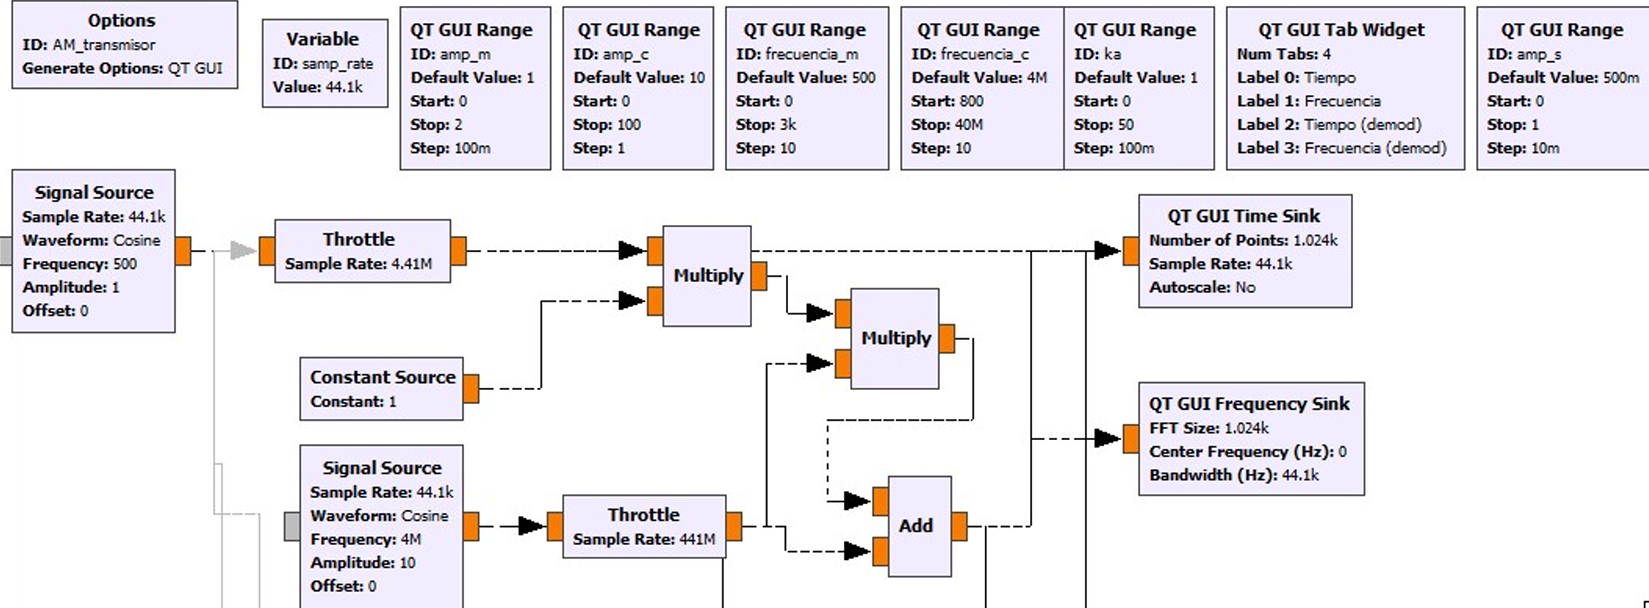
\includegraphics[width=0.7\textwidth]{imagenes/Parte_1/Actividad_6/fig3.png}
    \caption{Esquema del modulador AM en GNU Radio}
\end{figure}
